\begin{figure}[H]
    \centering
    \caption{How OPT performs when compared to an online algorithm LRU given the trace: A, B, C, D, A, B, C, C}
    \label{fig:my_label}
\begin{tikzpicture} 
    \node[rounded corners,draw=black,label=above:OPT, minimum size=2cm] (a) at (0,0)  {
    \begin{tikzpicture}
        \node[rounded corners,draw=black,minimum size=0.8cm]{A};
    \end{tikzpicture}
    
\begin{tikzpicture}
        \node[rounded corners,draw=black,minimum size=0.8cm]{};
    \end{tikzpicture}
    
\begin{tikzpicture}
        \node[rounded corners,draw=black,minimum size=0.8cm]{};
    \end{tikzpicture}
    };
    \node[text width=3cm] at (-3, 0) 
    {Miss on A, A added to cache};

    
    \node[rounded corners,draw=black,minimum size=2cm] (b) at (0,-2.5)  {   
\begin{tikzpicture}
        \node[rounded corners,draw=black,minimum size=0.8cm]{A};
    \end{tikzpicture}
    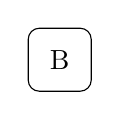
\begin{tikzpicture}
        \node[rounded corners,draw=black,minimum size=0.8cm]{B};
    \end{tikzpicture}
    
\begin{tikzpicture}
        \node[rounded corners,draw=black,minimum size=0.8cm]{};
    \end{tikzpicture}
    };
     \node[text width=3cm] at (-3,-2.5) 
    {Miss on B, B added to cache};
    
    \node[rounded corners,draw=black,minimum size=2cm] (c) at (0,-5)  {   
\begin{tikzpicture}
        \node[rounded corners,draw=black,minimum size=0.8cm]{A};
    \end{tikzpicture}
    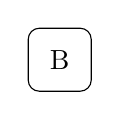
\begin{tikzpicture}
        \node[rounded corners,draw=black,minimum size=0.8cm]{B};
    \end{tikzpicture}
    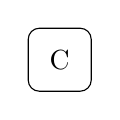
\begin{tikzpicture}
        \node[rounded corners,draw=black,minimum size=0.8cm]{C};
    \end{tikzpicture}
    };

    \node[text width=3cm] at (-3,-5) 
    {Miss on C, C added to cache};
      
    \node[rounded corners,draw=black,minimum size=2cm] (d) at (0,-7.5)  {   
\begin{tikzpicture}
        \node[rounded corners,draw=black,minimum size=0.8cm]{A};
    \end{tikzpicture}
    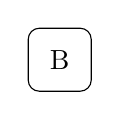
\begin{tikzpicture}
        \node[rounded corners,draw=black,minimum size=0.8cm]{B};
    \end{tikzpicture}
    
\begin{tikzpicture}
        \node[rounded corners,draw=black,minimum size=0.8cm]{D};
    \end{tikzpicture}
    };

     \node[text width=3cm] at (-3,-7.5) 
    {Miss on D, D added to cache, evict C since FITF};
    
    \node[rounded corners,draw=black,minimum size=2cm, below left=1 cm of d] (e) at (2.2,-8.4)  { 
    
\begin{tikzpicture}
        \node[rounded corners,draw=black,minimum size=0.8cm]{A};
    \end{tikzpicture}
    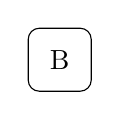
\begin{tikzpicture}
        \node[rounded corners,draw=black,minimum size=0.8cm]{B};
    \end{tikzpicture}
    
\begin{tikzpicture}
        \node[rounded corners,draw=black,minimum size=0.8cm]{D};
    \end{tikzpicture}
    };  

     \node[text width=3cm] at (-2.5,-9.8) 
    {Hit on A};
    
    \node[rounded corners,draw=black,minimum size=2cm,below left=1 cm of e] (f) at (2.2,-10.8)  { 
    
\begin{tikzpicture}
        \node[rounded corners,draw=black,minimum size=0.8cm]{A};
    \end{tikzpicture}
    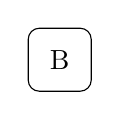
\begin{tikzpicture}
        \node[rounded corners,draw=black,minimum size=0.8cm]{B};
    \end{tikzpicture}
    
\begin{tikzpicture}
        \node[rounded corners,draw=black,minimum size=0.8cm]{D};
    \end{tikzpicture}
    };  

     \node[text width=3cm] at (-2.5,-12.2) 
    {Hit on B};

    
    \node[rounded corners,draw=black,minimum size=2cm, below left=1 cm of f] (g) at (2.2,-13.4)  { 
    
\begin{tikzpicture}
        \node[rounded corners,draw=black,minimum size=0.8cm]{A};
    \end{tikzpicture}
    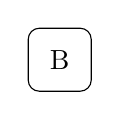
\begin{tikzpicture}
        \node[rounded corners,draw=black,minimum size=0.8cm]{B};
    \end{tikzpicture}
    
\begin{tikzpicture}
        \node[rounded corners,draw=black,minimum size=0.8cm]{D};
    \end{tikzpicture}
    };  

     \node[text width=3cm] at (-3,-14.7) 
    {Miss on C, evict D};
    
    \node[rounded corners,draw=black,minimum size=2cm, below left=1 cm of g] (h) at (2.2,-15.6)  { 
    
\begin{tikzpicture}
        \node[rounded corners,draw=black,minimum size=0.8cm]{A};
    \end{tikzpicture}
    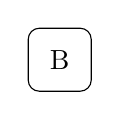
\begin{tikzpicture}
        \node[rounded corners,draw=black,minimum size=0.8cm]{B};
    \end{tikzpicture}
    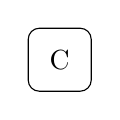
\begin{tikzpicture}
        \node[rounded corners,draw=black,minimum size=0.8cm]{C};
    \end{tikzpicture}
    }; 
    \node[text width=3cm] at (-2.5,-17.3) 
    {Hit on C};






















    %LRU
    \node[rounded corners,draw=black,label=above:LRU, minimum size=2cm] (i) at (6,0)  {
    
\begin{tikzpicture}
        \node[rounded corners,draw=black,minimum size=0.8cm]{A};
    \end{tikzpicture}
    
\begin{tikzpicture}
        \node[rounded corners,draw=black,minimum size=0.8cm]{};
    \end{tikzpicture}
    
\begin{tikzpicture}
        \node[rounded corners,draw=black,minimum size=0.8cm]{};
    \end{tikzpicture}
    };
    \node[text width=3cm] at (10,0) 
    {Miss on A, A added to cache};
    \node[text width=3cm] at (4,0) 
    {\Huge A};

    
    \node[rounded corners,draw=black,minimum size=2cm] (j) at (6,-2.5)  {   
\begin{tikzpicture}
        \node[rounded corners,draw=black,minimum size=0.8cm]{A};
    \end{tikzpicture}
    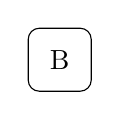
\begin{tikzpicture}
        \node[rounded corners,draw=black,minimum size=0.8cm]{B};
    \end{tikzpicture}
    
\begin{tikzpicture}
        \node[rounded corners,draw=black,minimum size=0.8cm]{};
    \end{tikzpicture}
    };
    \node[text width=3cm] at (10,-2.4) 
    {Miss on B, B added to cache};
    \node[text width=3cm] at (4,-2.4) 
    {\Huge B};
    
    \node[rounded corners,draw=black,minimum size=2cm] (k) at (6,-5)  {   
\begin{tikzpicture}
        \node[rounded corners,draw=black,minimum size=0.8cm]{A};
    \end{tikzpicture}
    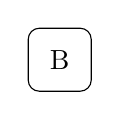
\begin{tikzpicture}
        \node[rounded corners,draw=black,minimum size=0.8cm]{B};
    \end{tikzpicture}
    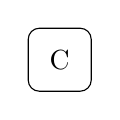
\begin{tikzpicture}
        \node[rounded corners,draw=black,minimum size=0.8cm]{C};
    \end{tikzpicture}
    };
    \node[text width=3cm] at (10,-4.8) 
    {Miss on C, C added to cache};
    \node[text width=3cm] at (4,-4.8) 
    {\Huge C};
    
      
    \node[rounded corners,draw=black,minimum size=2cm] (l) at (6,-7.5)  {   
\begin{tikzpicture}
        \node[rounded corners,draw=black,minimum size=0.8cm]{D};
    \end{tikzpicture}
    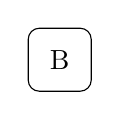
\begin{tikzpicture}
        \node[rounded corners,draw=black,minimum size=0.8cm]{B};
    \end{tikzpicture}
    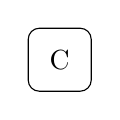
\begin{tikzpicture}
        \node[rounded corners,draw=black,minimum size=0.8cm]{C};
    \end{tikzpicture}
    };
     \node[text width=3cm] at (10,-7.4) 
    {Miss on D, Evict A as LRU};
    \node[text width=3cm] at (4,-7.4) 
    {\Huge D};

    
    \node[rounded corners,draw=black,minimum size=2cm, below left=1 cm of l] (m) at (8.2,-8.4)  { 
    
\begin{tikzpicture}
        \node[rounded corners,draw=black,minimum size=0.8cm]{D};
    \end{tikzpicture}
    
\begin{tikzpicture}
        \node[rounded corners,draw=black,minimum size=0.8cm]{A};
    \end{tikzpicture}
    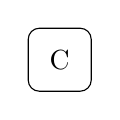
\begin{tikzpicture}
        \node[rounded corners,draw=black,minimum size=0.8cm]{C};
    \end{tikzpicture}
    };  
    \node[text width=3cm] at (10,-10) 
    {Miss on A, Evict B since LRU};
    \node[text width=3cm] at (4,-10) 
    {\Huge A};

    
    \node[rounded corners,draw=black,minimum size=2cm,below left=1 cm of m] (n) at (8.2,-10.8)  { 
    
\begin{tikzpicture}
        \node[rounded corners,draw=black,minimum size=0.8cm]{D};
    \end{tikzpicture}
    
\begin{tikzpicture}
        \node[rounded corners,draw=black,minimum size=0.8cm]{A};
    \end{tikzpicture}
    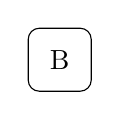
\begin{tikzpicture}
        \node[rounded corners,draw=black,minimum size=0.8cm]{B};
    \end{tikzpicture}
    };  
     \node[text width=3cm] at (10,-12.3) 
    {Miss on B, Evict C since LRU};
    \node[text width=3cm] at (4,-12.3) 
    {\Huge B};

    
    \node[rounded corners,draw=black,minimum size=2cm, below left=1 cm of n] (o) at (8.2,-13.4)  { 
    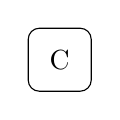
\begin{tikzpicture}
        \node[rounded corners,draw=black,minimum size=0.8cm]{C};
    \end{tikzpicture}
    
\begin{tikzpicture}
        \node[rounded corners,draw=black,minimum size=0.8cm]{A};
    \end{tikzpicture}
    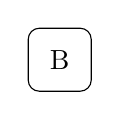
\begin{tikzpicture}
        \node[rounded corners,draw=black,minimum size=0.8cm]{B};
    \end{tikzpicture}
    };  
    \node[text width=3cm] at (10,-14.8) 
    {Miss on C, evict B};
    \node[text width=3cm] at (4,-14.8) 
    {\Huge C};
    
    
    \node[rounded corners,draw=black,minimum size=2cm, below left=1 cm of o] (p) at (8.2,-15.6)  { 
    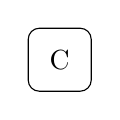
\begin{tikzpicture}
        \node[rounded corners,draw=black,minimum size=0.8cm]{C};
    \end{tikzpicture}
    
\begin{tikzpicture}
        \node[rounded corners,draw=black,minimum size=0.8cm]{A};
    \end{tikzpicture}
    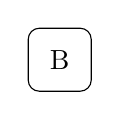
\begin{tikzpicture}
        \node[rounded corners,draw=black,minimum size=0.8cm]{B};
    \end{tikzpicture}
    };  
    \node[text width=3cm] at (10,-17.3) 
    {Hit on C};
    \node[text width=3cm] at (4,-17.3) 
    {\Huge C};

    \draw[thick,->] (a) -- (b);
    \draw[thick,->](b) -- (c);  
    \draw[thick,->](c) -- (d);  
    \draw[thick,->](d) -- (e);  
    \draw[thick,->] (e) -- (f);
    \draw[thick,->](f) -- (g);  
    \draw[thick,->](g) -- (h);
    
    \draw[thick,->] (i) -- (j);
    \draw[thick,->](j) -- (k);  
    \draw[thick,->](k) -- (l);  
    \draw[thick,->](l) -- (m);  
    \draw[thick,->] (m) -- (n);
    \draw[thick,->](n) -- (o);  
    \draw[thick,->](o) -- (p);
        
\end{tikzpicture}
\end{figure}